\begin{figure}
	\center
	\includegraphics[width=\linewidth]{vect/dataset_ex_hori}
%	\includegraphics[trim={0 10 0 0}, clip, width=\linewidth]{vect/dataset_ex}
	\caption{\label{fig:dataset} \textbf{Examples of test images :} we evaluate our proposal on four challenging localization sequences. The number under the query set name indicates the amount of query images to compare against the 1688 reference images.}
	\vspace{-0.25cm}
\end{figure}

\section{Experiments}
\label{sec:experiments}

\subsection{Dataset}
\label{subsec:dataset}
	We have tested our new method on the \textit{Oxford Robotcar} public dataset~\cite{Maddern2016}. This is a common dataset used for image-based localization~\cite{Sattler2018} and loop closure algorithm involving neural networks training~\cite{Porav2018}.
		
\vspace{4pt}\noindent\textbf{Training data.}
	We use the temporal redundancy present in the dataset to build the images triplets to train our CNN. We build 400 triplets using three runs acquired at dates: \texttt{2015-05-19, 2015-08-28} and \texttt{2015-11-10}. We selected an area of the city different from the one used for training our networks for validation.
	Depth modality is extracted from the lidar point cloud dataset of \textit{Oxford Robotcar}. When re-projected in the image frame coordinate, it produces a sparse depth map. Since deep convolutional neural networks require dense data as input, we pre-process these sparse modality maps with inpainting algorithm from~\cite{Bevilacqua2017} in order to make them dense.

\vspace{4pt}\noindent\textbf{Testing data.} We propose four testing scenarios on the same spatial area (different from the area used for training and validation). The reference dataset is composed of 1688 images taken every 5 meters along a path of 2 km, when the weather was overcast. The four query sets are:
\begin{itemize}
	\item {Sunny/Overcast:} queries have been acquired during a sunny day.
	\item {Long-term:} queries have been acquired 7 months after the reference images under similar weather conditions.
	\item {Winter/Summer:} queries have been acquired during a snowy day.
	\item {Night/Day:} queries have been acquired at night, resulting in radical visual changes compared to the reference images.
\end{itemize}

\noindent Query examples are presented in figure~\ref{fig:dataset}.
	
\vspace{4pt}\noindent\textbf{Evaluation metric.} For a given query, the reference images are ranked according to the cosine similarity score computed over their descriptors. To evaluate the localization performances, we consider two evaluation metrics:
	\setcounter{paragraph}{0}

	\paragraph{Recall @N} we plot the percentage of well localized queries regarding the number $N$ of returned candidates. A query is considered well localized if one of the top $N$ retrieved images lies inside the $25m$ radius of the ground truth query position.
	\paragraph{Top-1 recall @D} We compute the distance between the top ranked returned database image position and the query ground truth position, and report the percentage of queries located under a threshold $D$ (from 15 to 50 meters), like in~\cite{Zamir2014}. This metric qualifies the accuracy of the localization system.

\subsection{Implementation details}
\label{subsec:implementation}

Our proposal is implemented by using Pytorch as deep learning framework, ADAM stochastic gradient descent algorithm for the CNN training with learning rate set to 1e-4, weight decay to 1e-3 and $\lambda$ in triplet loss equal to 0.1. We use batch size between 10 and 25 triplets depending of the size of the system to train, convergence occurs rapidly and takes around 30 to 50 epochs. We perform both positive and negative hard mining, as in~\cite{Radenovic2017}. Images and depth maps are re-sized to $224\times224$ pixels before training and testing.

\vspace{4pt}\noindent\textbf{Encoder architectures.} We test the fully convolutional part of Alexnet and Resnet18 architectures for features extraction. The size of the final features block is $256\times13\times13$ for Alexnet and $512\times7\times7$ for Resnet. Initial weights are the ones obtained by training the whole network on ImageNet dataset. We always use Alexnet encoder to extract features from raw depth map, reconstructed depth map, or hallucinated depth map. Indeed the quality of our depth map is usually very low, we have found that using deeper network does not significantly improve localization results.

\vspace{4pt}\noindent\textbf{Descriptor architectures.} We test the two state-of-the-art image descriptors MAC~\cite{Radenovic2017} and NetVLAD~\cite{Arandjelovic2017}. MAC is a simple global pooling method that takes the maximum of each feature map from the encoder output. NetVLAD is a trainable pooling layer that mimics VLAD aggregation method. For all the experiments, we set the number of NetVLAD clusters to 64. Finally, both MAC and NetVLAD descriptors are $L_{2}$ normalized.

\vspace{4pt}\noindent\textbf{Decoder architecture.} The decoder used in our proposal is based on Unet architecture and inspired by network generator from~\cite{Isola2017}. Dimension up-sampling is performed through inverse-convolutions layers. Decoder weights are initialized randomly.

\subsection{Results}
\label{subsec:results}

\begin{figure}
	\center
	\begin{minipage}{0.49\linewidth}
		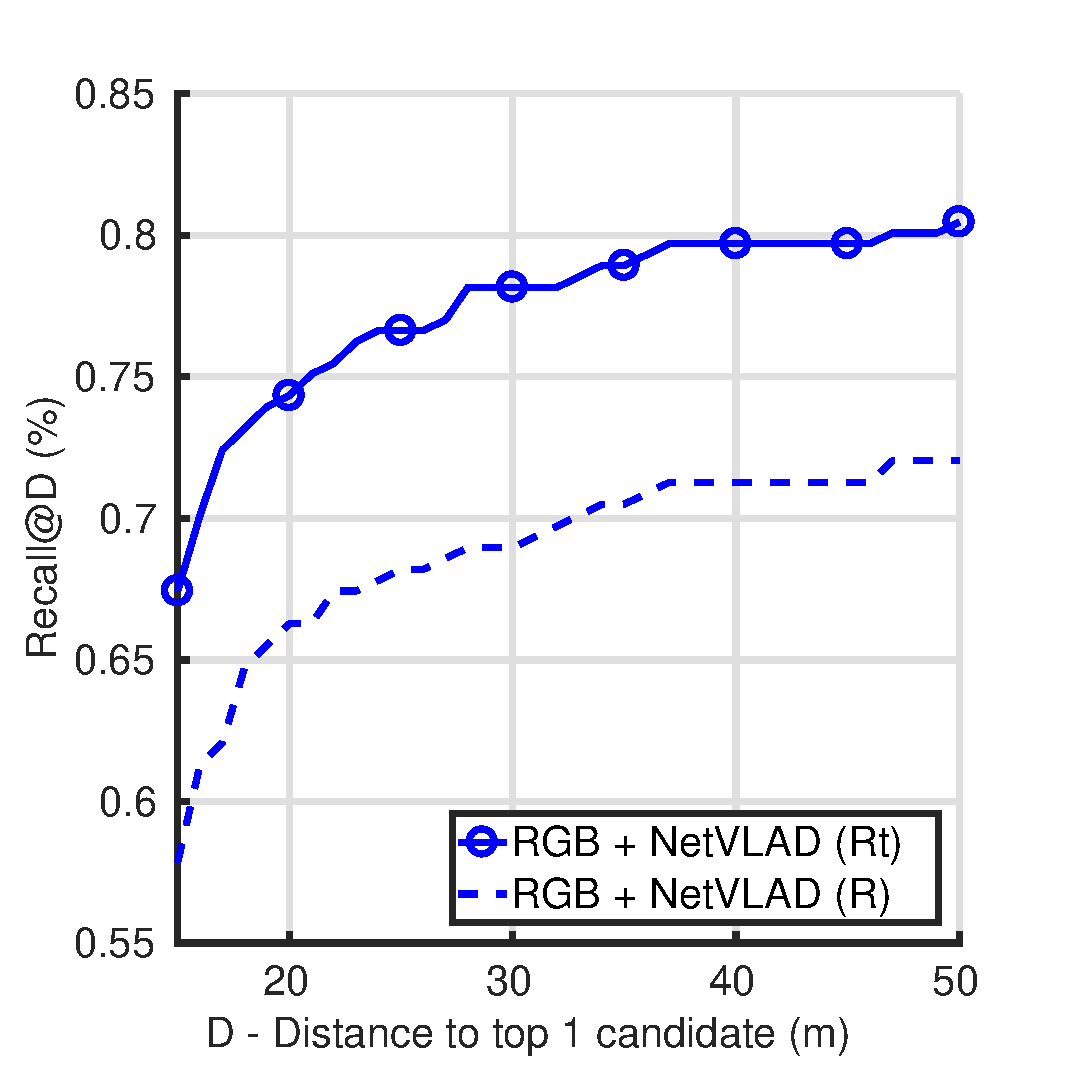
\includegraphics[width=\linewidth]{plot/fig/rgb_r_trunc_distance}	
	\end{minipage}
	\begin{minipage}{0.49\linewidth}
		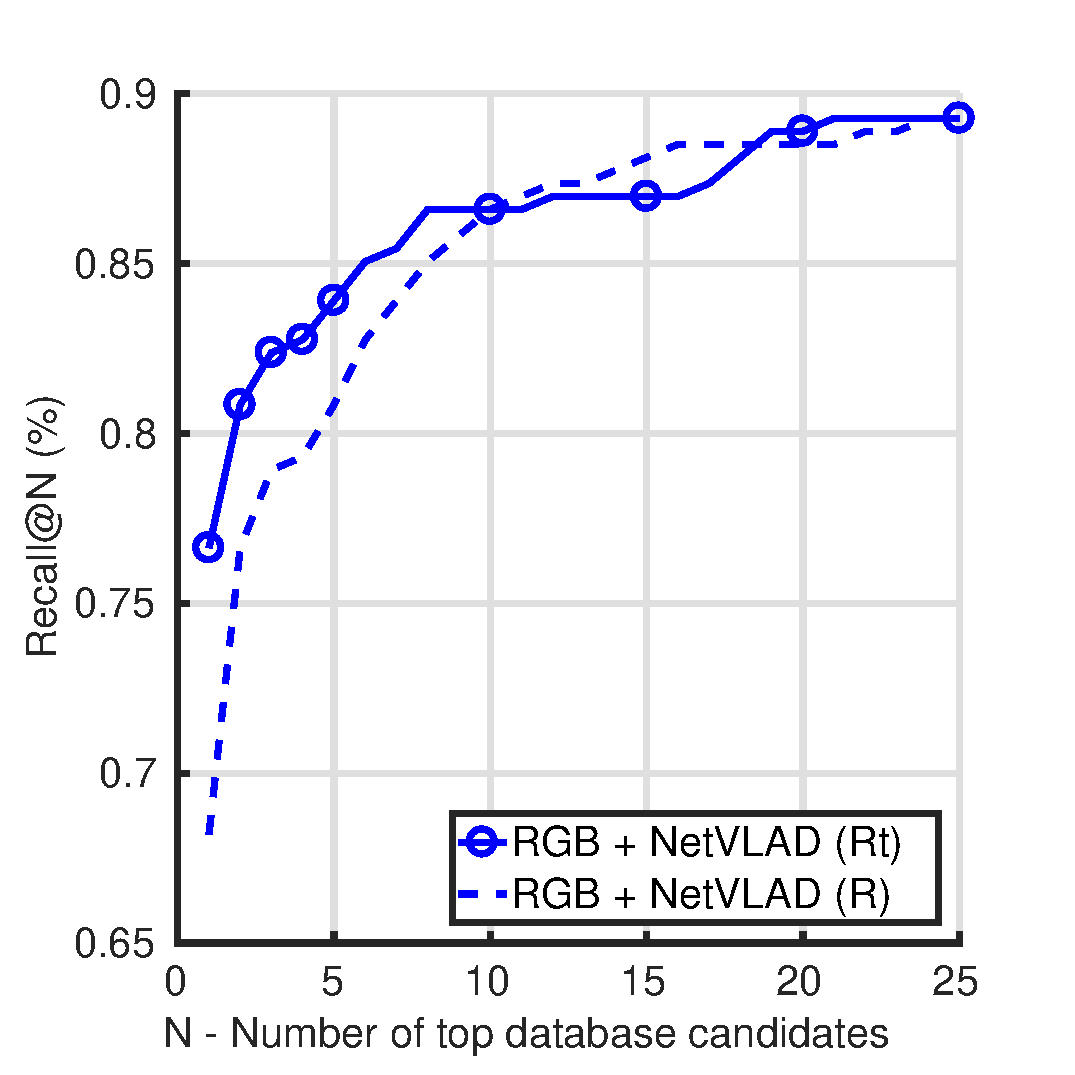
\includegraphics[width=\linewidth]{plot/fig/rgb_r_trunc_recall}	
	\end{minipage}
	\caption{\label{fig:trunc_resnet} \textbf{Resnet18 (R) versus truncated Resnet18 (Rt) in combination with NetVLAD pooling:} we show the importance of the spatial resolution of the deep feature maps of the encoder used with NetVLAD layer. The truncated version of Resnet18, more than two times lighter than the complete one, achieves much better localization results.}
	\vspace{-0.25cm}
\end{figure}

\begin{figure*}
	\center
	\begin{minipage}{0.14\linewidth}
		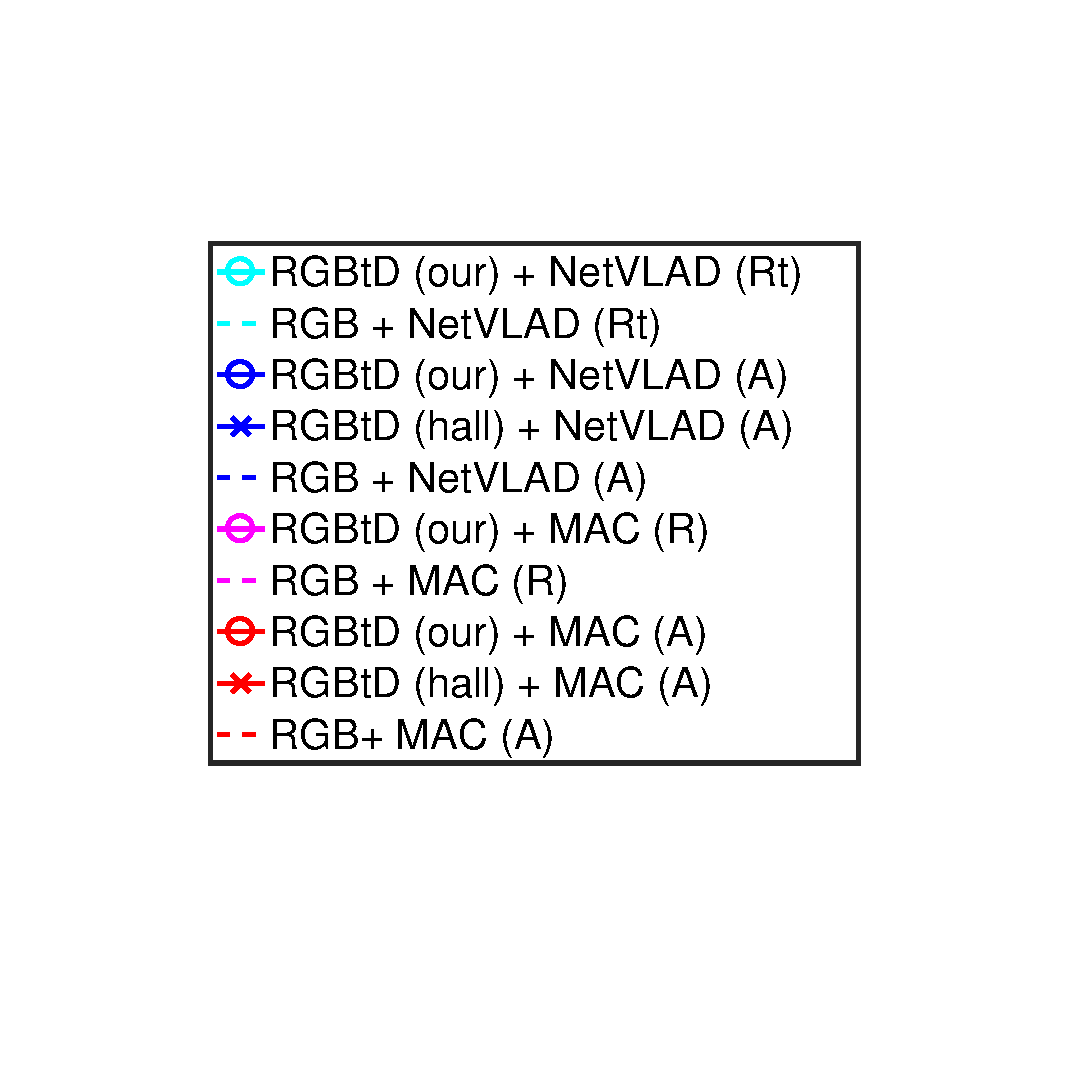
\includegraphics[trim={90 140 95 100},clip,width=\linewidth]{plot/fig/legend}	
	\end{minipage}
	\begin{minipage}{0.85\linewidth}
	
	\begin{minipage}{0.49\linewidth}		
		\center
		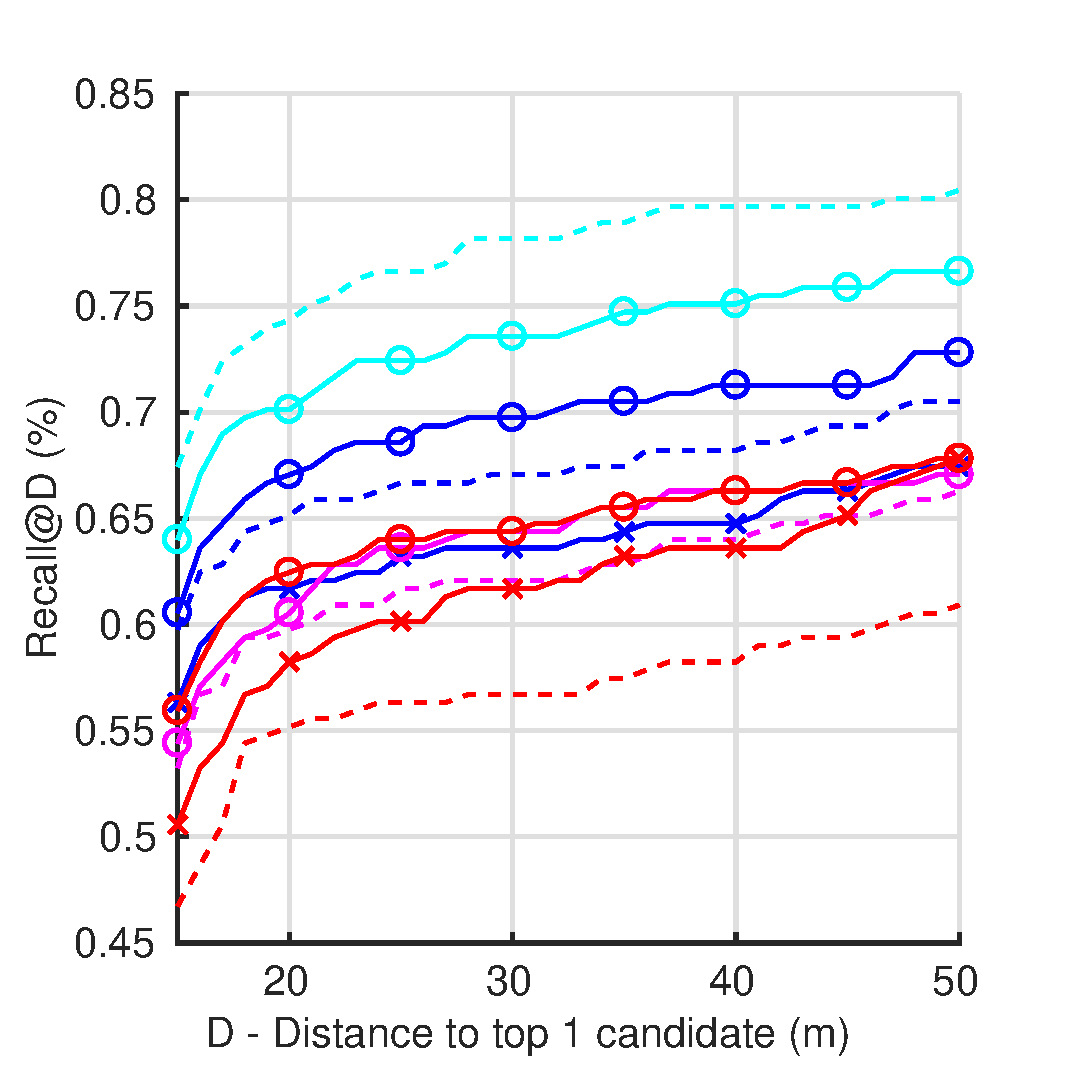
\includegraphics[width=0.49\linewidth]{plot/fig/sun_distance}	
		\includegraphics[width=0.49\linewidth]{plot/fig/sun_recall}
		
		{\scriptsize a) Sunny/Overcast}
	\end{minipage}
	\begin{minipage}{0.49\linewidth}
		\center
		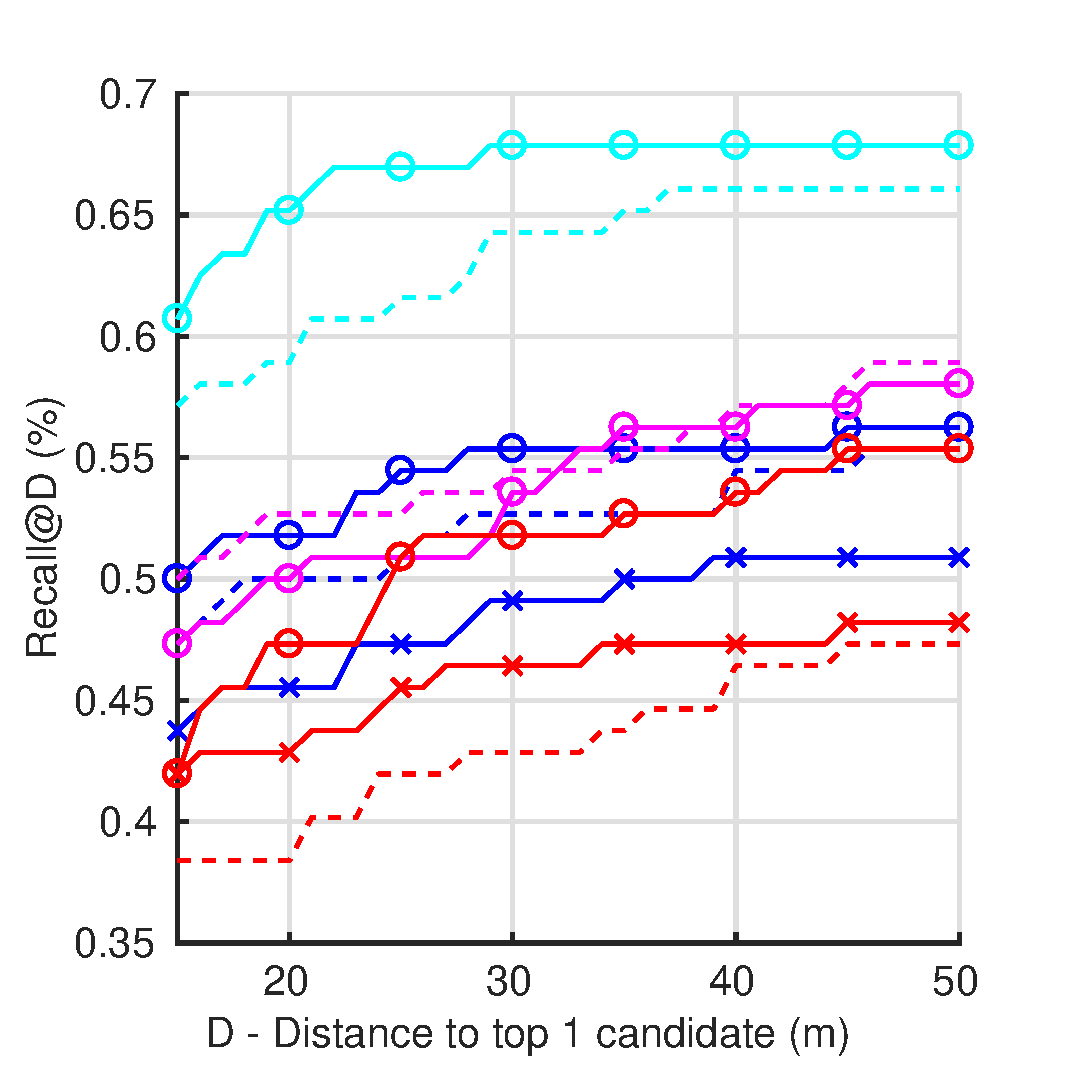
\includegraphics[width=0.49\linewidth]{plot/fig/snow_distance}	
		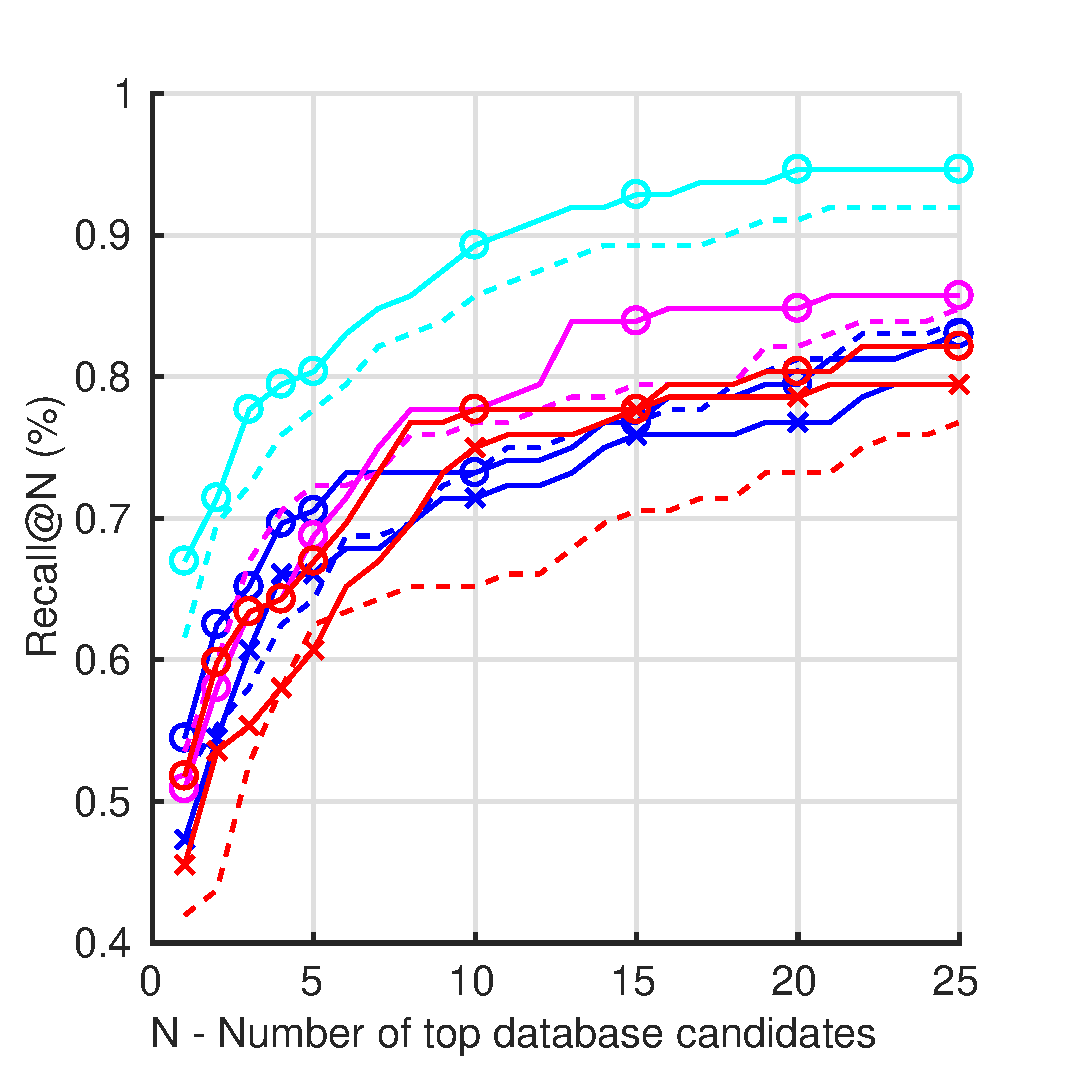
\includegraphics[width=0.49\linewidth]{plot/fig/snow_recall}
		
		{\scriptsize b) Winter/Summer}
	\end{minipage}
	
	\begin{minipage}{0.49\linewidth}
		\center
		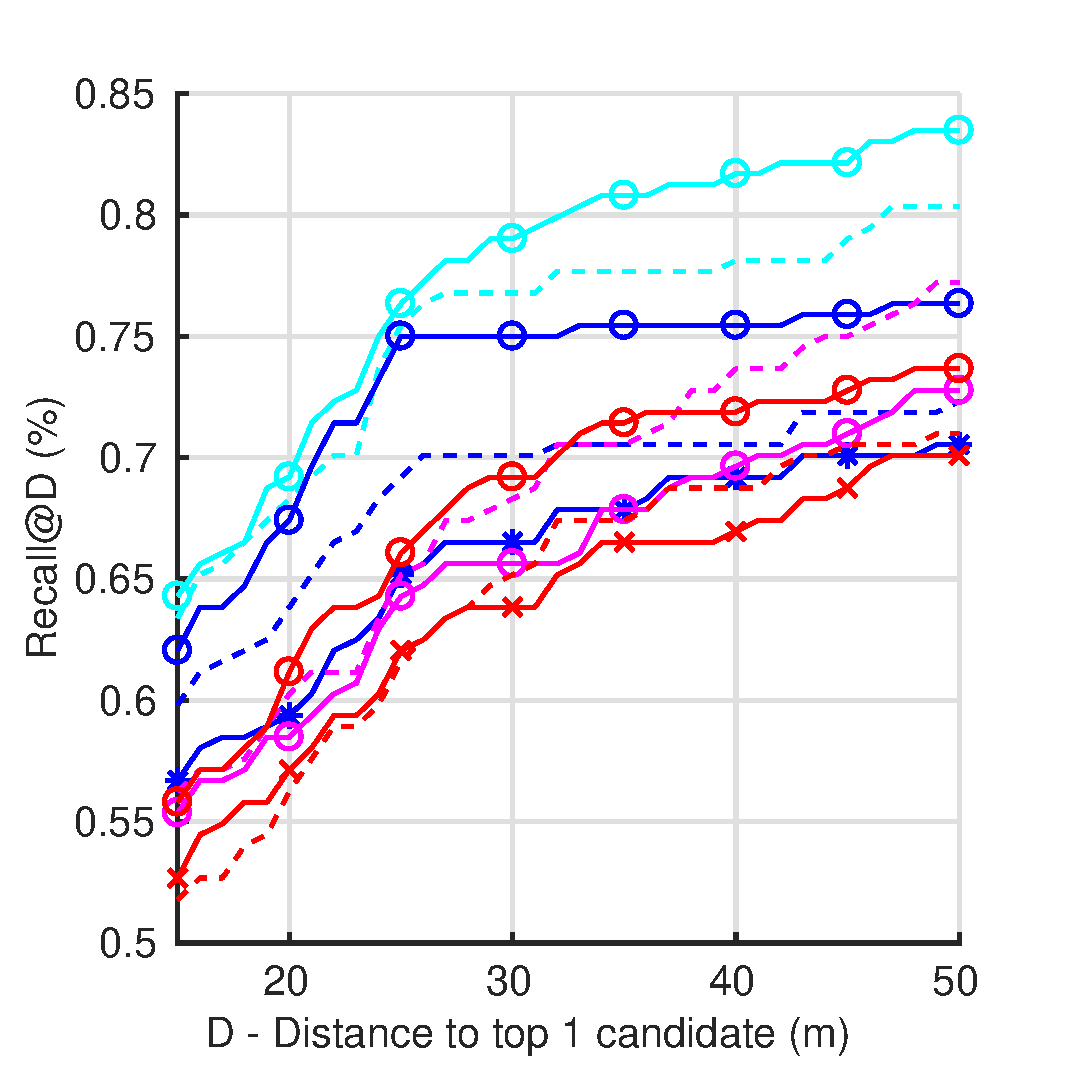
\includegraphics[width=0.49\linewidth]{plot/fig/lt_distance}	
		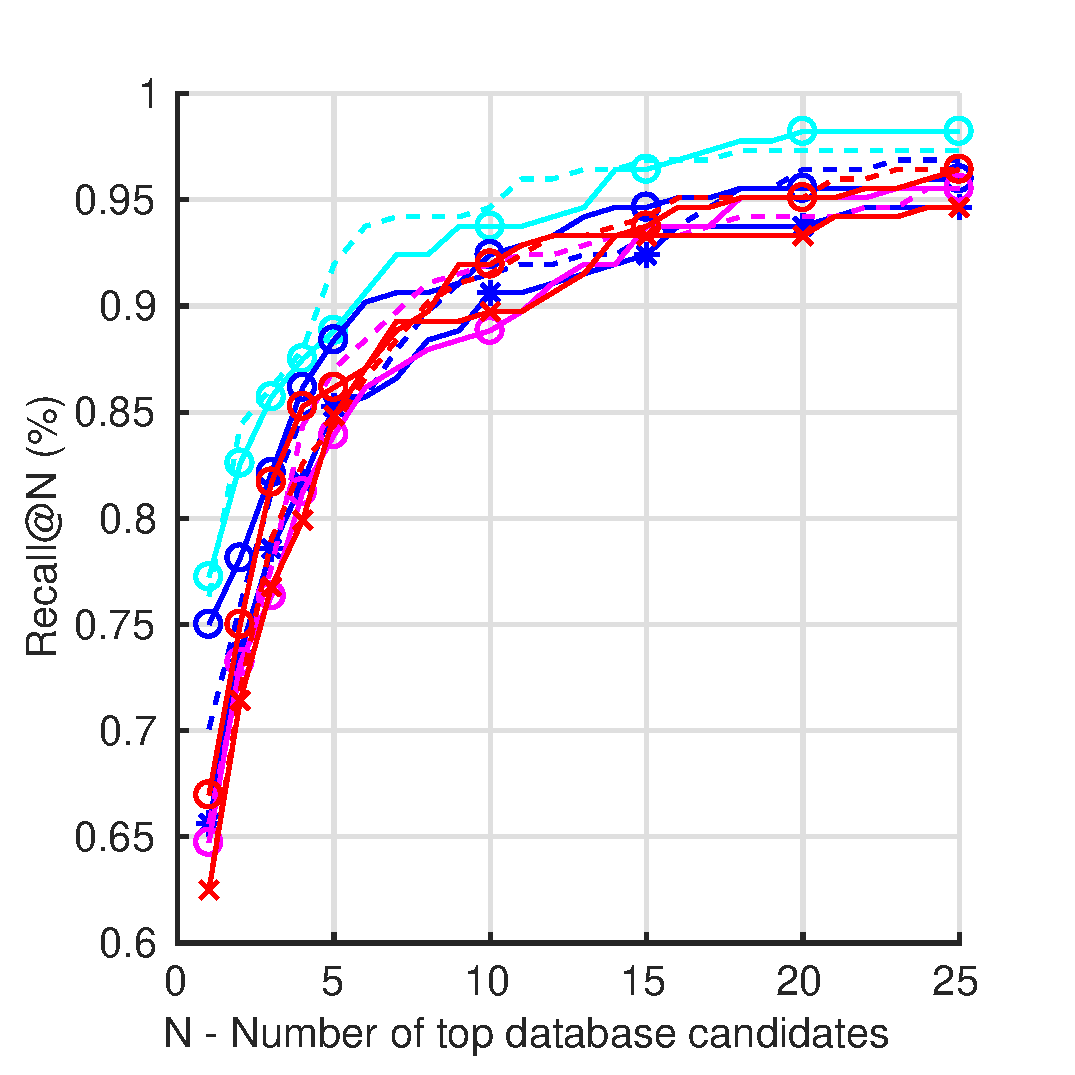
\includegraphics[width=0.49\linewidth]{plot/fig/lt_recall}

		{\scriptsize c) Long-term}		
	\end{minipage}
	\begin{minipage}{0.49\linewidth}
		\center	
		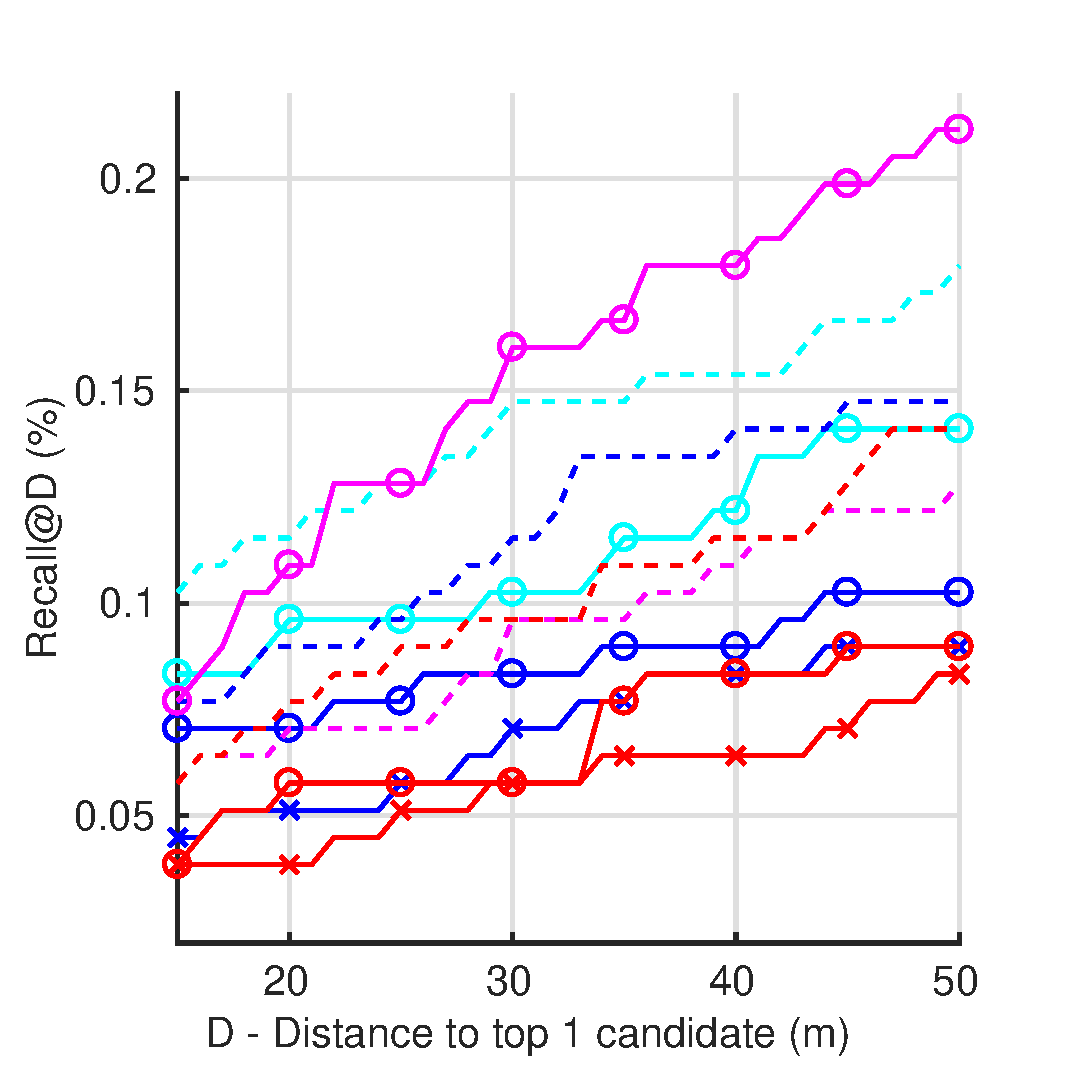
\includegraphics[width=0.49\linewidth]{plot/fig/night_distance}	
		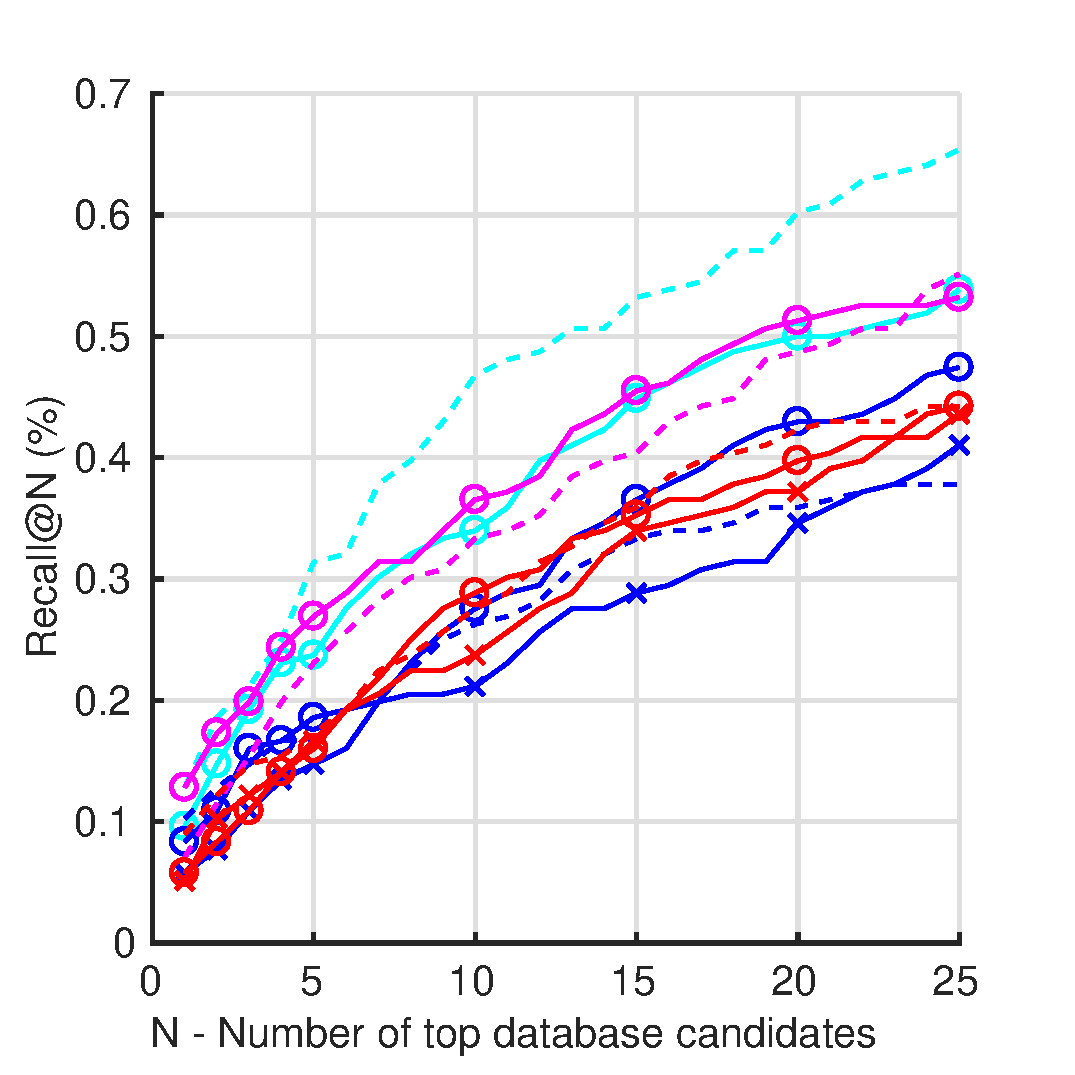
\includegraphics[width=0.49\linewidth]{plot/fig/night_recall}
	
		{\scriptsize d) Night/Day}
	\end{minipage}
	
	\end{minipage}

	\caption{\label{fig:results} \textbf{Comparison of our method versus hallucination network and networks trained with only images}: our method (-o-) is superior in almost every scenario facing hallucination network (-x-). It also beats, with a significant margin, networks trained with only images (\texttt{--}). NetVLAD descriptors (\textcolor{blue}{blue} and \textcolor{cyan}{cyan} curves) are superior to MAC (\textcolor{red}{red} and \textcolor{magenta}{magenta} curves), specially in terms of accuracy (Recall@D curve). Night/day dataset remains the most challenging one. Curves best viewed in colors.}
	\vspace{-0.25cm}
\end{figure*}

\noindent\textbf{Baselines.} We compare our method with two state-of-the-art baselines:
    \paragraph{RGB only (\textbf{RGB})} simple networks composed of encoder + descriptor trained with only images, without side depth maps information. We evaluate 4 variants of networks, by combining Alexnet (A) or Resnet (R) encoder with MAC or NetVLAD descriptor pooling.
    \paragraph{RGB with Depth side information (\textbf{RGBtD})} networks that use pairs of aligned image and depth map during training step and images only at test time. We compare our proposal with our version of hallucination network~\cite{Hoffman2016} (hall). We follow training procedure of~\cite{Hoffman2016} to train the hallucination network, whereas our proposal is trained as explained in~\ref{subsec:training}. 

\vspace{4pt}\noindent\textbf{Truncated Resnet.} We experimented that NetVLAD descriptor combined with Resnet architecture, RGB + NetVLAD (R), does not perform well. NetVLAD can be view as a pooling method that acts on local deep features densely extracted from the input image. We argue that the spatial resolution of the features block obtained with Resnet encoder is too low compared to the other architecture (for instance $13\times13$ for Alexnet compared to $7\times7$ for Resnet for an $224\times224$ input image). We propose a truncated version of Resnet encoder (Rt), created by drooping the end of the network after the 13th convolutional layer. Thus we obtain a feature block with greater spatial resolution: $256\times14\times14$ compared to $512\times7\times7$. Recall results on the \textit{Sunny/Overcast} query set for both architectures are presented in figure~\ref{fig:trunc_resnet}. As the truncated version of Resnet encoder clearly dominates the full one, we use the truncated version for the following experiments.

\vspace{4pt}\noindent\textbf{Discussion.} 
{
\setlength{\tabcolsep}{1.3pt}
\renewcommand{\arraystretch}{1.2}
\begin{table}
	\caption{\label{tab/sum_res} Results top-1 recall @D: MAC (A) \& NetVLAD (Rt).}
	\scriptsize \center
	\begin{tabular}{l l | c c c | c c c | c c c | c c c}
	\multicolumn{2}{c|}{\multirow{2}{0.8cm}{Methods}} & \multicolumn{3}{c|}{Sunny} & \multicolumn{3}{c|}{Long-term} & \multicolumn{3}{c|}{Winter} & \multicolumn{3}{c}{All} \\
	 	&	  & @15   & @25   & @50   & @15   & @25  & @50   & @15   & @25   & @50   & @15 & @25 & @50 \\
	\hline
%	\textit{Baseline} & MAC & 46.7 & 56.3 & 60.9 & 51.8 & 62.5 & 71.0 & 38.4 & 42.0 & 47.3 & 45.6 & 53.6 & 59.7 \\
%	\textit{(A)	}				 	 & NetVLAD	& 59.8 & 66.7 & 70.1 & 59.8 & 70.1 & 72.3 & 47.3 & 51.8 & 55.4 & 55.6 & 62.9 & 65.9 \\
%	\textit{Baseline} & MAC & 53.3 & 61.7 & 66.3 & 56.3 & 65.8 & 77.2 & 50.0 & 51.8 & 58.9 & 53.2 & 59.8 & 67.5 \\
%	\textit{(R)}						 & NetVLAD  & 67.4 & 76.6 & 80.5 & 63.4 & 76.3 & 80.4 & 57.1 & 61.6 & 66.1 & 62.6 & 71.5 & 75.6 \\
	\multirow{2}{0.5cm}{\textit{RGB}} & MAC  & 46.7 & 56.3 & 60.9 & 51.8 & 62.5 & 71.0 & 38.4 & 42.0 & 47.3 & 45.6 & 53.6 & 59.7 \\
									 & NetVLAD   & 67.4 & 76.6 & 80.5 & 63.4 & 76.3 & 80.4 & 57.1 & 61.6 & 66.1 & 62.6 & 71.5 & 75.6 \\
	\multicolumn{2}{l|}{\textbf{Mean (all RGB)}} & 56.8 & 65.3 & 69.4 & 57.8 & 68.7 & 75.2 & 48.2 & 51.8 & 56.9 & \textbf{54.3} & \textbf{61.9} & \textbf{67.2} \\
	\hline
%	\textit{Our} 	  & MAC & 55.9 & 64.0 &	67.8 & 55.8 & 67.0 & 73.7 &	42.0 & 51.8 & 55.4 & 51.2 & 60.9 & 65.6 \\
%	\textit{(A)}  & NetVLAD & 60.5 & 69.4 &	72.8 & 62.1 & 75.0 & 76.3 &	50.0 & 54.5 & 56.3 & 57.5 & 66.8 & 68.4 \\
%	\textit{Our} & 		MAC & 54.4 & 63.6 & 67.1 & 55.4 & 64.7 & 72.8 &	47.3 & 50.9	& 58.0 & 52.3 & 59.7 & 66.0 \\
%	\textit{(R)} & 	NetVLAD & 64.0 & 72.4 &	76.6 & 64.3 & 77.2 & 83.5 & 60.7 & 67.0 & 67.9 & 63.0 & 72.2 & 76,0 \\
	\multirow{2}{0.5cm}{\textit{Our}} &		MAC  & 55.9 & 64.0 &	67.8 & 55.8 & 67.0 & 73.7 &	42.0 & 51.8 & 55.4 & 51.2 & 60.9 & 65.6 \\
									& 	NetVLAD & 64.0 & 72.4 &	76.6 & 64.3 & 77.2 & 83.5 & 60.7 & 67.0 & 67.9 & 63.0 & 72.2 & 76,0 \\	
	\multicolumn{2}{l|}{\textbf{Mean (all our)}} 	& 58.7 & 67.3 & 71.1 & 59.4 & 71.0 & 76.6 & 50.0 & 56.0 & 59.4 & \textbf{56.0} & \textbf{64.8} & \textbf{69.0} \\	
	\hline
	\end{tabular}
	\vspace{-0.25cm}
\end{table}
}
Localization results on the four query sets are presented in figure~\ref{fig:results}. Both method trained with auxiliary depth information (hall and our) perform on average better than the RGB baseline. This shows that the geometric clues given during the training process can be efficiently used for the task of image-only retrieval for localization. Compare to hallucination network, our method shows better results, both in term of recall and precision. We report results for the hallucination network only with encoder Alexnet as we were not able to obtain stable training when using a deeper architecture. 

We also report on table~\ref{tab/sum_res} localization performances for the 3 day-time datasets (sunny, long-term and winter). We obtain our best localization results by combining truncated Resnet base encoder with NetVLAD descriptor. However, for all combination of encode/decoder, our method increases the localization precision compare to the RGB baseline. This demonstrate the generalization capability of our method: we can either use lightweight architecture for online embedded localization or rely on greedier models to increase the overall localization precision. Our method only decreases the localization performances compare to the baseline when using Resnet+NetVLAD on the sunny/overcast query set. This is certainly because the training data are visually similar to the queries present in this scenario. It will be interesting to introduce attention mechanism to balance the relative importance of image and depth modality to overcome this problem.

Our method shows the best localization improvement on the Winter/Summer query set. Standard image descriptors are confused by local changes caused by the snow present on the scene whereas our descriptor remains confident by reconstructing the geometric structure of the scene. Similar results should be intended regarding Night/Day query sets (figure~\ref{fig:results}-d), however our proposal is not able to improve localization accuracy for this query set. We investigate the night to day localization scenario in the following.

\vspace{4pt}\noindent\textbf{Night to day localization.} Night to day localization is an extremely challenging problem: our best RGB baseline achieves less than 13\% recall@1. This can be explained by the huge difference in visual appearance between night and daytime images, as illustrated in figure~\ref{fig:dataset}. Our system should be able to improve the RGB baseline relying on the learned scene geometry, which remains the same during day and night. Unfortunately, we use training data exclusively composed of daytime images, thus making the decoder unable to reconstruct a depth map from an image taken at night. The last line of figure~\ref{fig:mod_ex} shows the poor quality of decoder output after initial training. In order to improve the decoder's performances, we propose to use weakly annotated data to fine tune the decoder part of our system. We collect 1000 pairs of image and depth map acquired at night and retrain only decoder weights $\theta_G$ using loss of equation~(\ref{eq:l1_loss}). Figure~\ref{fig:mod_ex} presents the qualitative amelioration on the inferred depth map after the fine tuning. Such post-processing trick cannot be used to improve standard RGB image descriptors, because we need to know the location of the night data. For instance, we use a night run from the Robotcar dataset with a low quality GPS signal, that makes impossible the automatic creation of triplets that are essential for training a deep image descriptor. We show in figure~\ref{fig:ft_night} that we are able to nearly multiply by two the localization performances by only fine tuning a small part of our system. Our best network achieves 23\% recall@1 against 13\% recall@1 for the best RGB baseline.

\vspace{4pt}\noindent\textbf{Contribution of the depth information.} In this paragraph, we investigate the impact on localization performances provided by the side geometry information on our method. To ensure a fair comparison in terms of number of trainable parameters, we introduce RGB$^+$ network that has the same architecture as our proposed method. We train RGB$^+$ with images only to compare the localization results against our method that uses side depth information. For training RGB$^+$, we simply remove the loss introduced in equation~(\ref{eq:generator}), and make the weights of the decoder trainable when optimizing triplets losses constraints. Results of this experiment with encoder architecture Alexnet are presented in table~\ref{tab/eval_depth}.

{
\setlength{\tabcolsep}{5pt}
\renewcommand{\arraystretch}{1.2}
\begin{table}
	\caption{\label{tab/eval_depth} Contribution of the depth side information during training.}
	\scriptsize \center
	\begin{tabular}{c  | c  c | c  c  c | c  c}
	\multirow{2}{0.8cm}{\textbf{Query}\\\textbf{set}} & \multicolumn{2}{c|}{\textbf{Network}} & \multicolumn{3}{c|}{\textbf{Top-1 recall@D}} & \multicolumn{2}{c}{\textbf{Recall@N}} \\
	\cline{2-8}
	              								& Name & \#Param.  	& @15 & @30 & @50 & @1 & @5\\
	\hline
	\multirow{3}{0.8cm}{Sunny/\\Overcast} & RGB + MAC &  2.5M		& 46.7 & 56.7 & 60.9 & 56.3 & 76.6 \\
										  & RGB$^{+}$ + MAC & 7.9M	& 51.0 & 61.0 & 66.7 & 60.1 &  79.3 \\  
										  & RGBtD + MAC &  7.9M	& \textbf{55.9} & \textbf{64.4} & \textbf{67.8} & \textbf{64.0} &  \textbf{80.5} \\
   \hline
   	\multirow{3}{0.8cm}{Long-\\term} & RGB + MAC & 2.5M			& 51.8 & 65.2 & 71.0 & 62.5 &  84.4 \\
									 & RGB$^{+}$ + MAC & 7.9M		& 54.5 & 68.3 & 72.3 & \textbf{67.0} & 82.6  \\  
									 & RGBtD + MAC & 7.9M			& \textbf{55.8} & \textbf{69.2} & \textbf{73.7} & \textbf{67.0} & \textbf{86.2} \\
   \hline
	\multirow{3}{0.8cm}{Winter/\\Summer} & RGB + MAC & 2.5M		& 38.4 & 43.0 & 47.3 & 42.0 & 62.5 \\
										 & RGB$^{+}$ + MAC & 7.9M	& 36.6 & 42.0 & 43.0 & 41.1 & 56.3 \\  
										 & RGBtD + MAC & 7.9M		& \textbf{42.0} & \textbf{51.8} & \textbf{55.4} & \textbf{51.8} & \textbf{67.0} \\
   \hline

	\end{tabular}
\end{table}
}

Increasing the size of the system results in a better localization on the two easiest query sets. Surprisingly RGB$^{+}$ system decreases localization performances on the winter queries compared to RGB. The system has probably over-fitted on the training data that are visually close to queries of ``Sunny" set and ``Long-term" set, but quiet different from the queries of ``Winter" set (see figure~\ref{fig:dataset}). Our RGBtD + MAC system always produces higher localization results facing RGB$^{+}$ + MAC, which shows that the side depth information provided during training is wisely used to describe the image location. 

\begin{figure}
	\center
	\includegraphics[trim={0 15 0 0},clip,width=\linewidth]{vect/mod_ex}	
	\caption{\label{fig:mod_ex} \textbf{Effect of fine tuning with night images on decoder output:}. Decoder trained with daylight images is unable to reconstruct the scene geometry (bottom line). Fine tuning the network with less than 1000 pairs \{image, depth map\} acquired by night highly improves appearance of the generated depth maps. Maps best viewed in color.}
	\vspace{-0.25cm}
\end{figure}

\begin{figure}
	\center
	\begin{minipage}{0.49\linewidth}
		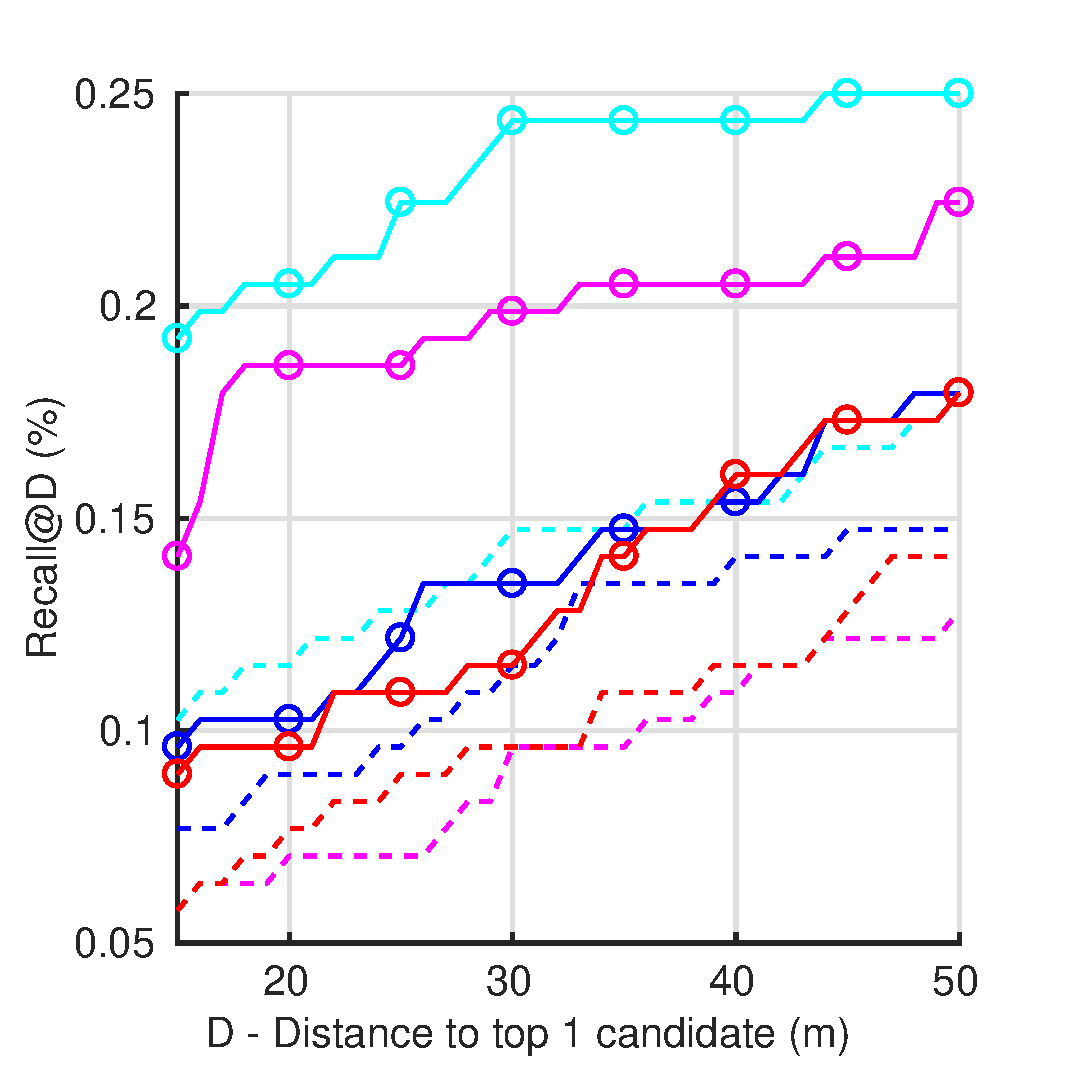
\includegraphics[width=\linewidth]{plot/fig/nightft_distance}	
	\end{minipage}
	\begin{minipage}{0.49\linewidth}
		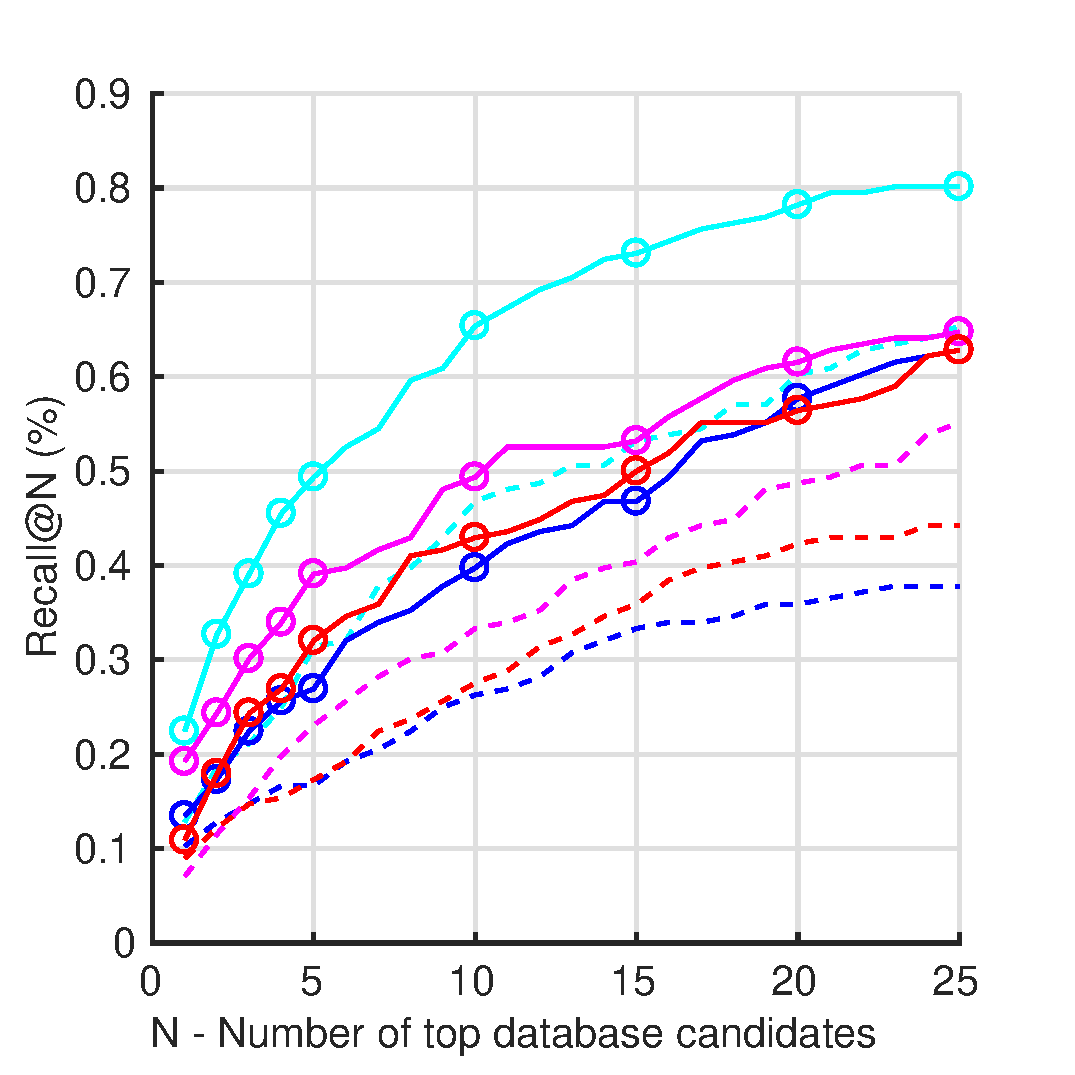
\includegraphics[width=\linewidth]{plot/fig/nightft_recall}	
	\end{minipage}
	\vspace{0.2cm}
	
	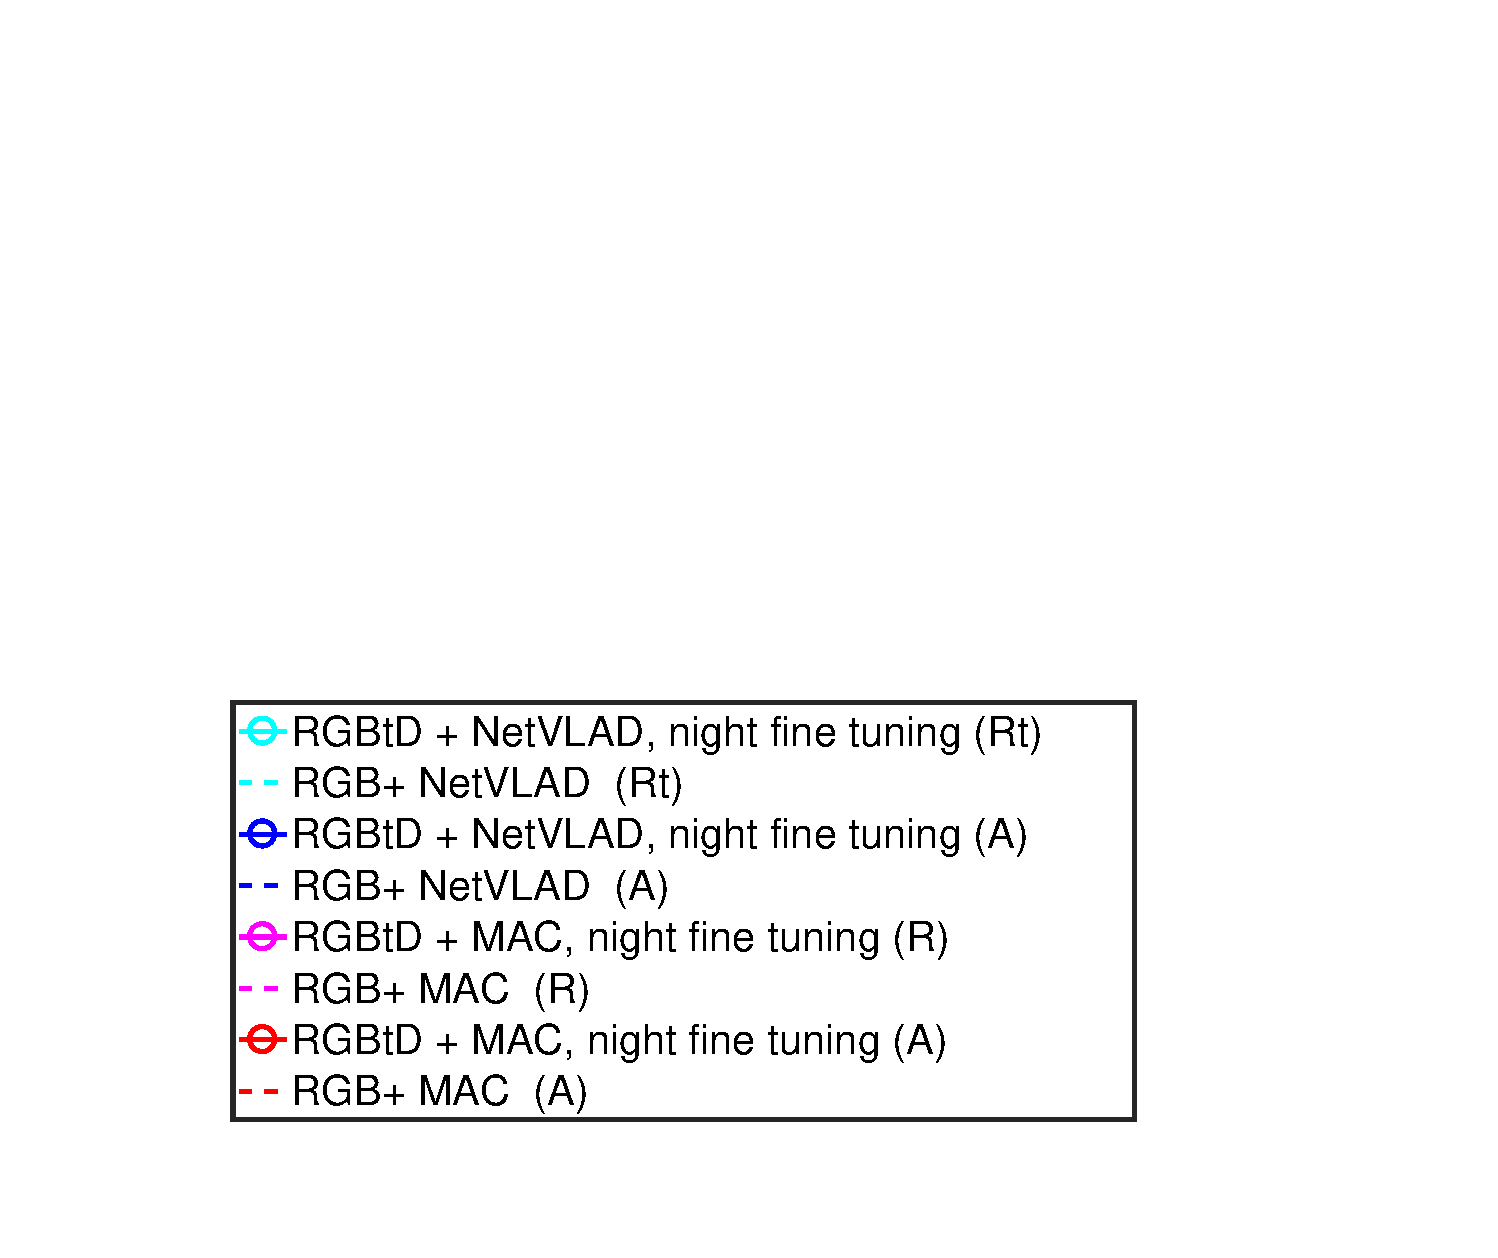
\includegraphics[trim={108 160 205 335},clip,width=0.4\linewidth]{plot/fig/legend_night_corr}\hspace{0.1cm}
	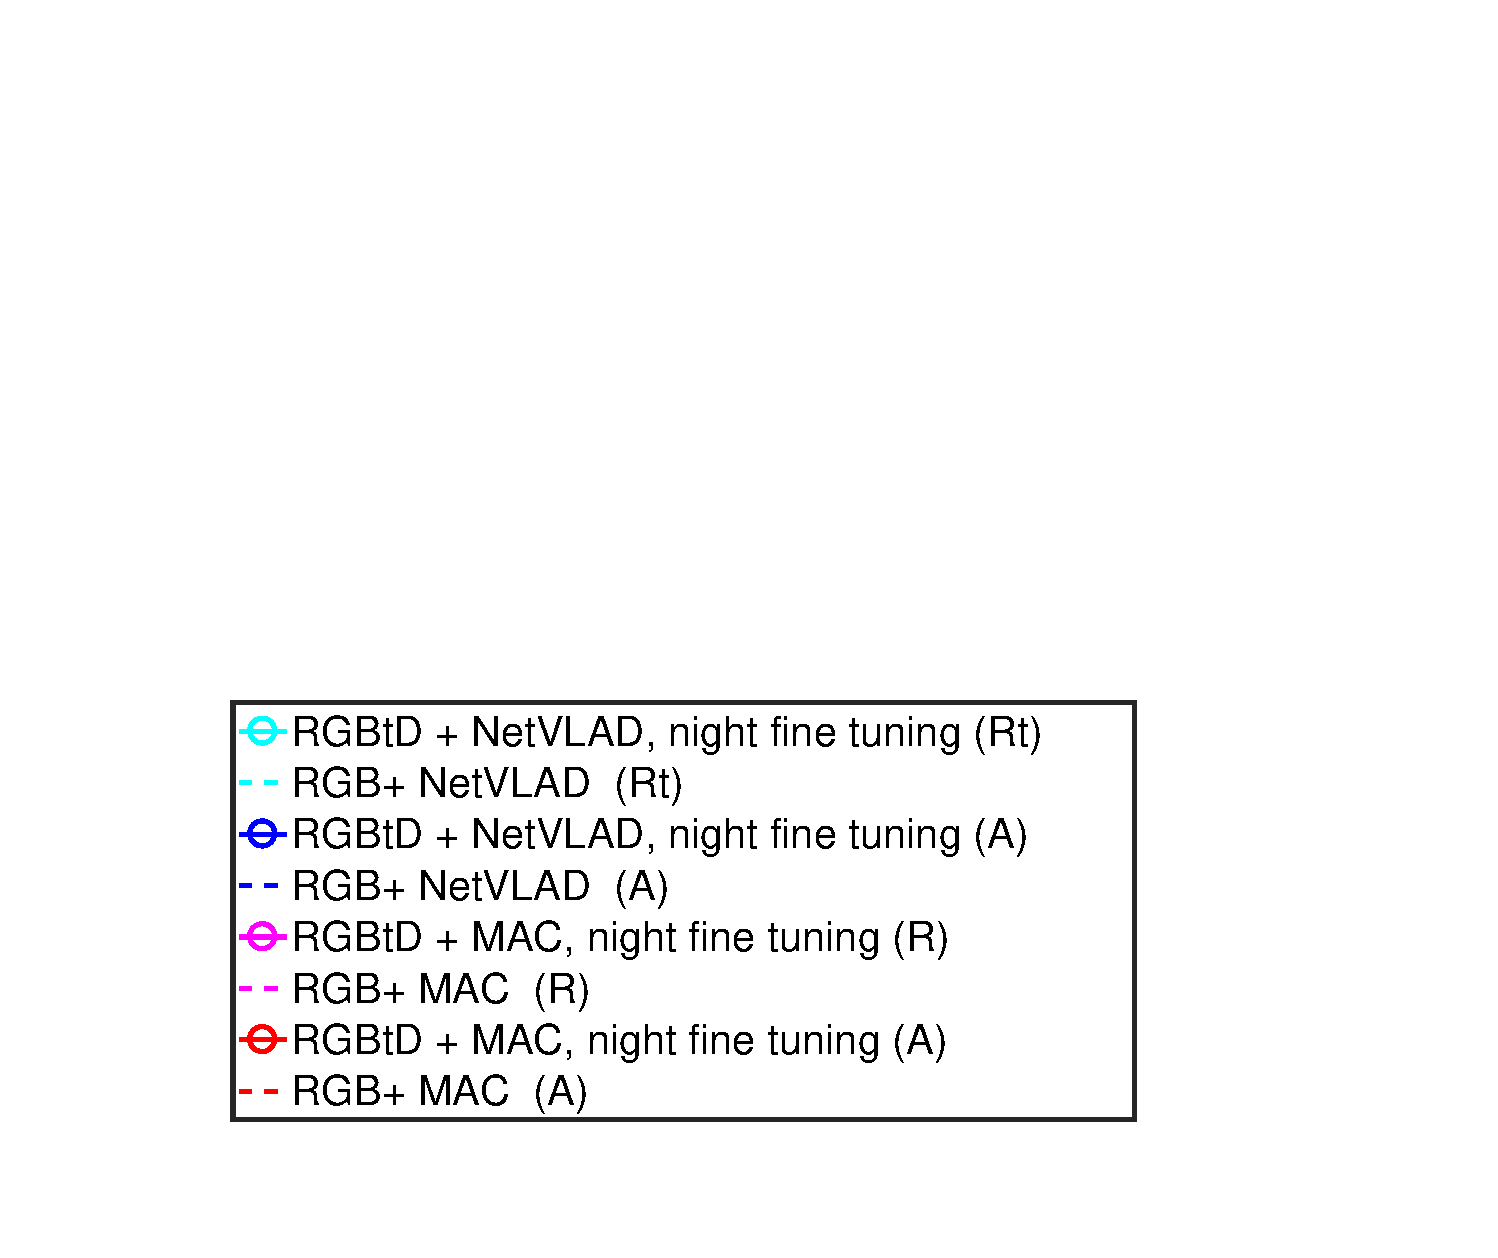
\includegraphics[trim={108 60 205 430},clip,width=0.4\linewidth]{plot/fig/legend_night_corr}
	\caption{\label{fig:ft_night} \textbf{Results on Night/Day query set after fine tuning:} we are able to drastically improve localization performance for the Night/Day challenging scenario by only fine tuning the decoder part of our network with weakly annotated data. Curves best viewed in color.}
	\vspace{-0.25cm}
\end{figure}
